As chapter \ref{s:map-scale} on page \ref{s:map-scale} already mentioned, the map scale is heavily dependent on the map projection. The true figure of the earth is not a regular shape like a sphere or an ellipsoid. It has a seperate shape, which is called geoid.
From a general point of view, every projection distorts the earth somehow, but the advantage of projection is, that any point can be exactly recreated at any given time, due to the fact, that the projection affects the whole earth.
A projection consists of four main properties:
\begin{enumerate*}
\item area,
\item form,
\item distance and
\item directions.
\end{enumerate*}
Every projection affects all its properties in some way. Some of them preserve area and form while distorting distances and directions \iacite{Snyder1987}.

In order to understand the sub-chapters explaining different types of projections, some terms need to be explained first:

\begin{enumerate}

\ditem{Conformal} \hfill \\
If a projection is conformal, it preserves local angles in the map. This can be thought of preserving the general shape of e.g. an island. Some parts of an island may get larger or smaller due to a conformal projection, but the recognizability of the island is still given \iacite{Snyder1987}.

\ditem{Loxodromes} \hfill \\
According to the Merriam Webster Online Dictionary\footnote{See \href{http://www.merriam-webster.com/}{Merriam Webster Dictionary}} a loxodrome is also called rhumb line and can be defined as "[\ldots] a line on the surface of the earth that follows a single compass bearing and makes equal oblique angles with all meridians". A more practical example of loxodromes is to imagine a sailing route between two points. This line is shown as a straight line, as long as the intended course of the ship remains constant with respect to north.

\ditem{Equal-Area} \hfill \\
If a map bares the name equal-area, it means that it preserves area by distorting shapes.

\end{enumerate}

For most thematic maps irregularities of the earth's shape are ignored, as long as geodetic accuracy is not related to the purpose of the map \iacite{Snyder1987}. Figure \ref{fig:projections-base} on page \ref{fig:projections-base} is in the subsections and helps to explain some major characteristics of the different types of projections. Every projection is only listed with its characteristics. These will not be discussed in detail, as it would go beyond the scope of this thesis.

\begin{figure}[!htb]
\centering
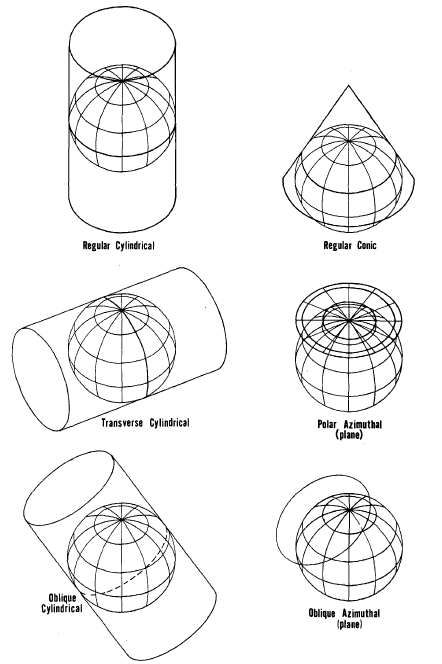
\includegraphics[width=0.8\textwidth,keepaspectratio]{images/methods/mappings.png}
\caption[
    Projection of the earth onto the three major surfaces \iacite{Snyder1987}.
]{Projection of the earth onto the three major surfaces.}
\label{fig:projections-base}
\end{figure}

\subsubsubsection{Cylindrical map projections}
The main concept of cylindrical map projections consist "[\ldots] of meridians which are equidistant parallel straight lines, crossed at right angles by straight parallel lines of latitude, generally not equidistant \iacite{Snyder1987}".
In general, cylindrical map projections can be thought of unrolling a cylinder which has been wrapped around a geoid, touching at the equator (see figure \ref{fig:projections-base} on page \pageref{fig:projections-base}).
The primary use for this type of projection is to either map the complete world, or for maps along narrow strips of a great circlel arc, such as the equator.

The following list will only feature two common projections accordingly to cylindrical projections with a short description taken from \citeauthor{Snyder1987} \iacite{Snyder1987}:

\begin{enumerate}

\ditem{Mercator Projection} \hfill \\
It is a cylindrical, conformal projection where meridians are equally spaced straight lines, whereas parallels are unequally spaced straight lines. The scale of the map is only true along the equator and loxodromes are straight lines. The biggest distortion appears close to the poles. The major advantage according to \citeauthor{Snyder1987} is the navigational feature that loxodromes are straight lines \iacite{Snyder1987}. Figure \ref{fig:projections-mercator} on page \pageref{fig:projections-mercator} shows an example mercator projection of the earth.

\begin{figure}[!htb]
\centering
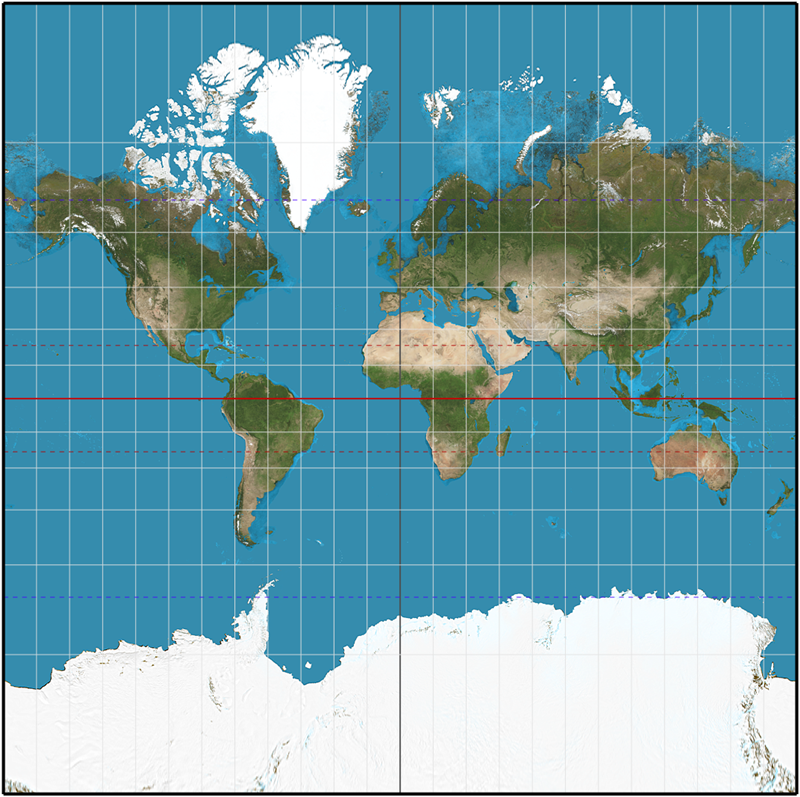
\includegraphics[height=5cm,keepaspectratio]{images/methods/projections/mercator.png}
\caption[
    Mercator projection, Urldate: 07.2016 \newline
    \small\texttt{\url{https://upload.wikimedia.org/wikipedia/commons/f/f0/MercNormSph.png}}.
]{Mercator projection}
\label{fig:projections-mercator}
\end{figure}


\ditem{Transverse Mercator Projection} \hfill \\
This projection is similar to the basic mercator projection except the main difference of a transverse, cylindrical and conformal projection. The central meridian and each meridian 90 degrees east and west of the central meridian are straight lines. All other meridians and parallels are complex curves. The scale of the map is only true along the central meridian \iacite{Snyder1987}. Figure \ref{fig:projections-mercator-transverse} on page \pageref{fig:projections-mercator-transverse} illustrates the described characteristics.

\begin{figure}[!htb]
\centering
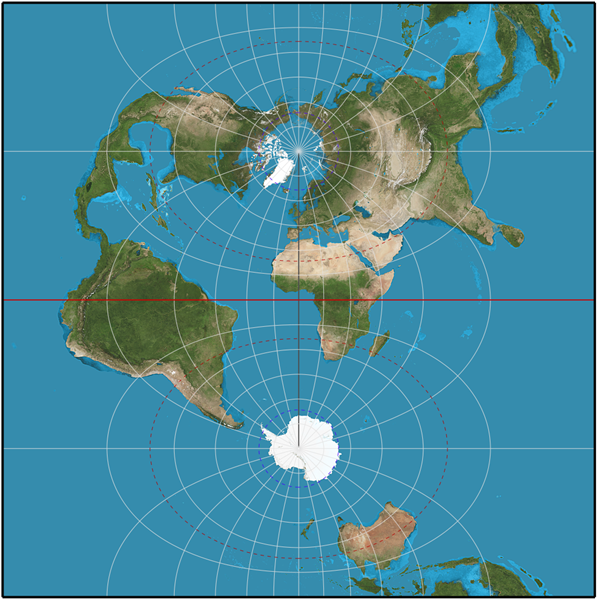
\includegraphics[height=5cm,keepaspectratio]{images/methods/projections/mercator-transverse.png}
\caption[
    Transverse mercator projection, Urldate: 07.2016 \newline
    \small\texttt{\url{https://upload.wikimedia.org/wikipedia/commons/1/15/MercTranSph.png}}.
]{Mercator projection}
\label{fig:projections-mercator-transverse}
\end{figure}


\end{enumerate}

\subsubsubsection{Conic map projections}
Conic projections are preferred over cylindrical ones if the purpose of the map is to show a region for which the greatest areal extent is from east to west in the temperature zone. This projection type makes use of "[\ldots] arcs of concentric circles for parallels of latitude and equally spaced straight radii of these circles for meridians \iacite{Snyder1987}." The main distinctive feature is based on placing a cone on the top of a globe representing the earth (see figure \ref{fig:projections-base} on page \pageref{fig:projections-base}).

The following list will only feature two common projections with a short description taken from \citeauthor{Snyder1987} \iacite{Snyder1987}:

\begin{enumerate}
\ditem{Albers Equal-Area Projection} \hfill \\
This projection, as seen in figure \ref{fig:projections-albers-ea} on page \pageref{fig:projections-albers-ea}, is a conic, area-preserving one where parallels are unequally spaced arcs of concentric circles, whereas meridians are equally spaced radii of the same circles. It features no distortion in scale or shape along two standard parallels, normally, or along just one. Both poles are arcs of circles. The projection is used for regions with predominant east-west expanse \iacite{Snyder1987}.

\begin{figure}[!htb]
\centering
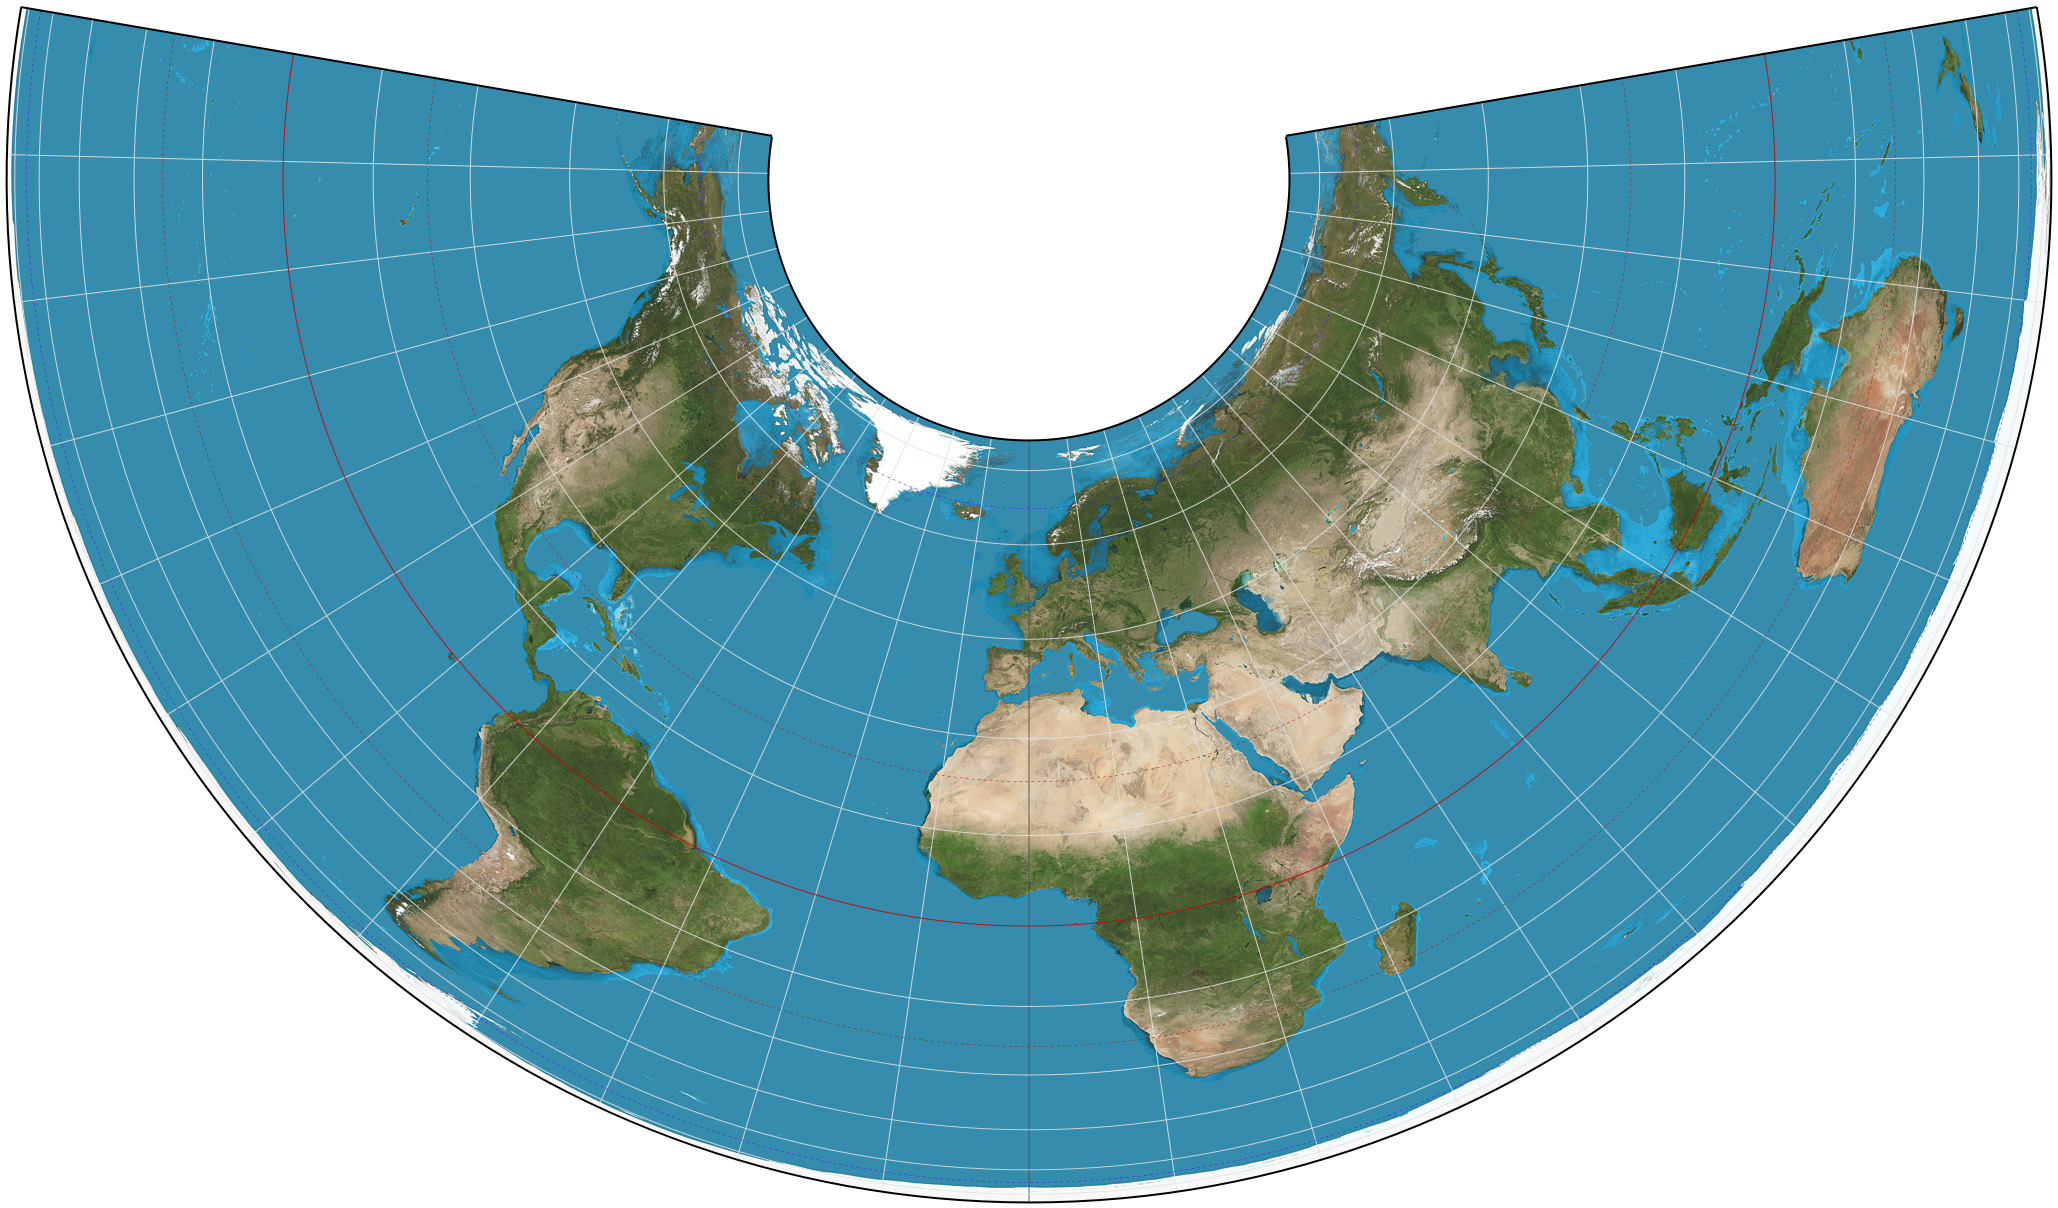
\includegraphics[height=5cm,keepaspectratio]{images/methods/projections/albers.jpg}
\caption[
    Albers equal-area projection, Urldate: 07.2016 \newline
    \small\texttt{\url{https://upload.wikimedia.org/wikipedia/commons/1/1f/Albers_projection_SW.jpg}}.
]{Albers equal-area projection}
\label{fig:projections-albers-ea}
\end{figure}

\ditem{Equidistant Conic Projection} \hfill \\
Equidistant conic projection displays parallels, including poles, as arcs of concentric circles evenly spaced along the meridians. Like the albers equal-area projection, equidistant projection also displays meridians as equally spaced radii of the same circles and thereby cutting parallels at right angles. The scaling of the map is true along all meridians and along one or two standard parallels \iacite{Snyder1987}. Figure \ref{fig:projections-equidistant} on page \pageref{fig:projections-equidistant} shows similarities to the albers equal-area projection. The major distinction is the distortion of direction, area and shape according to the distance from standard parallels.

\begin{figure}[!htb]
\centering
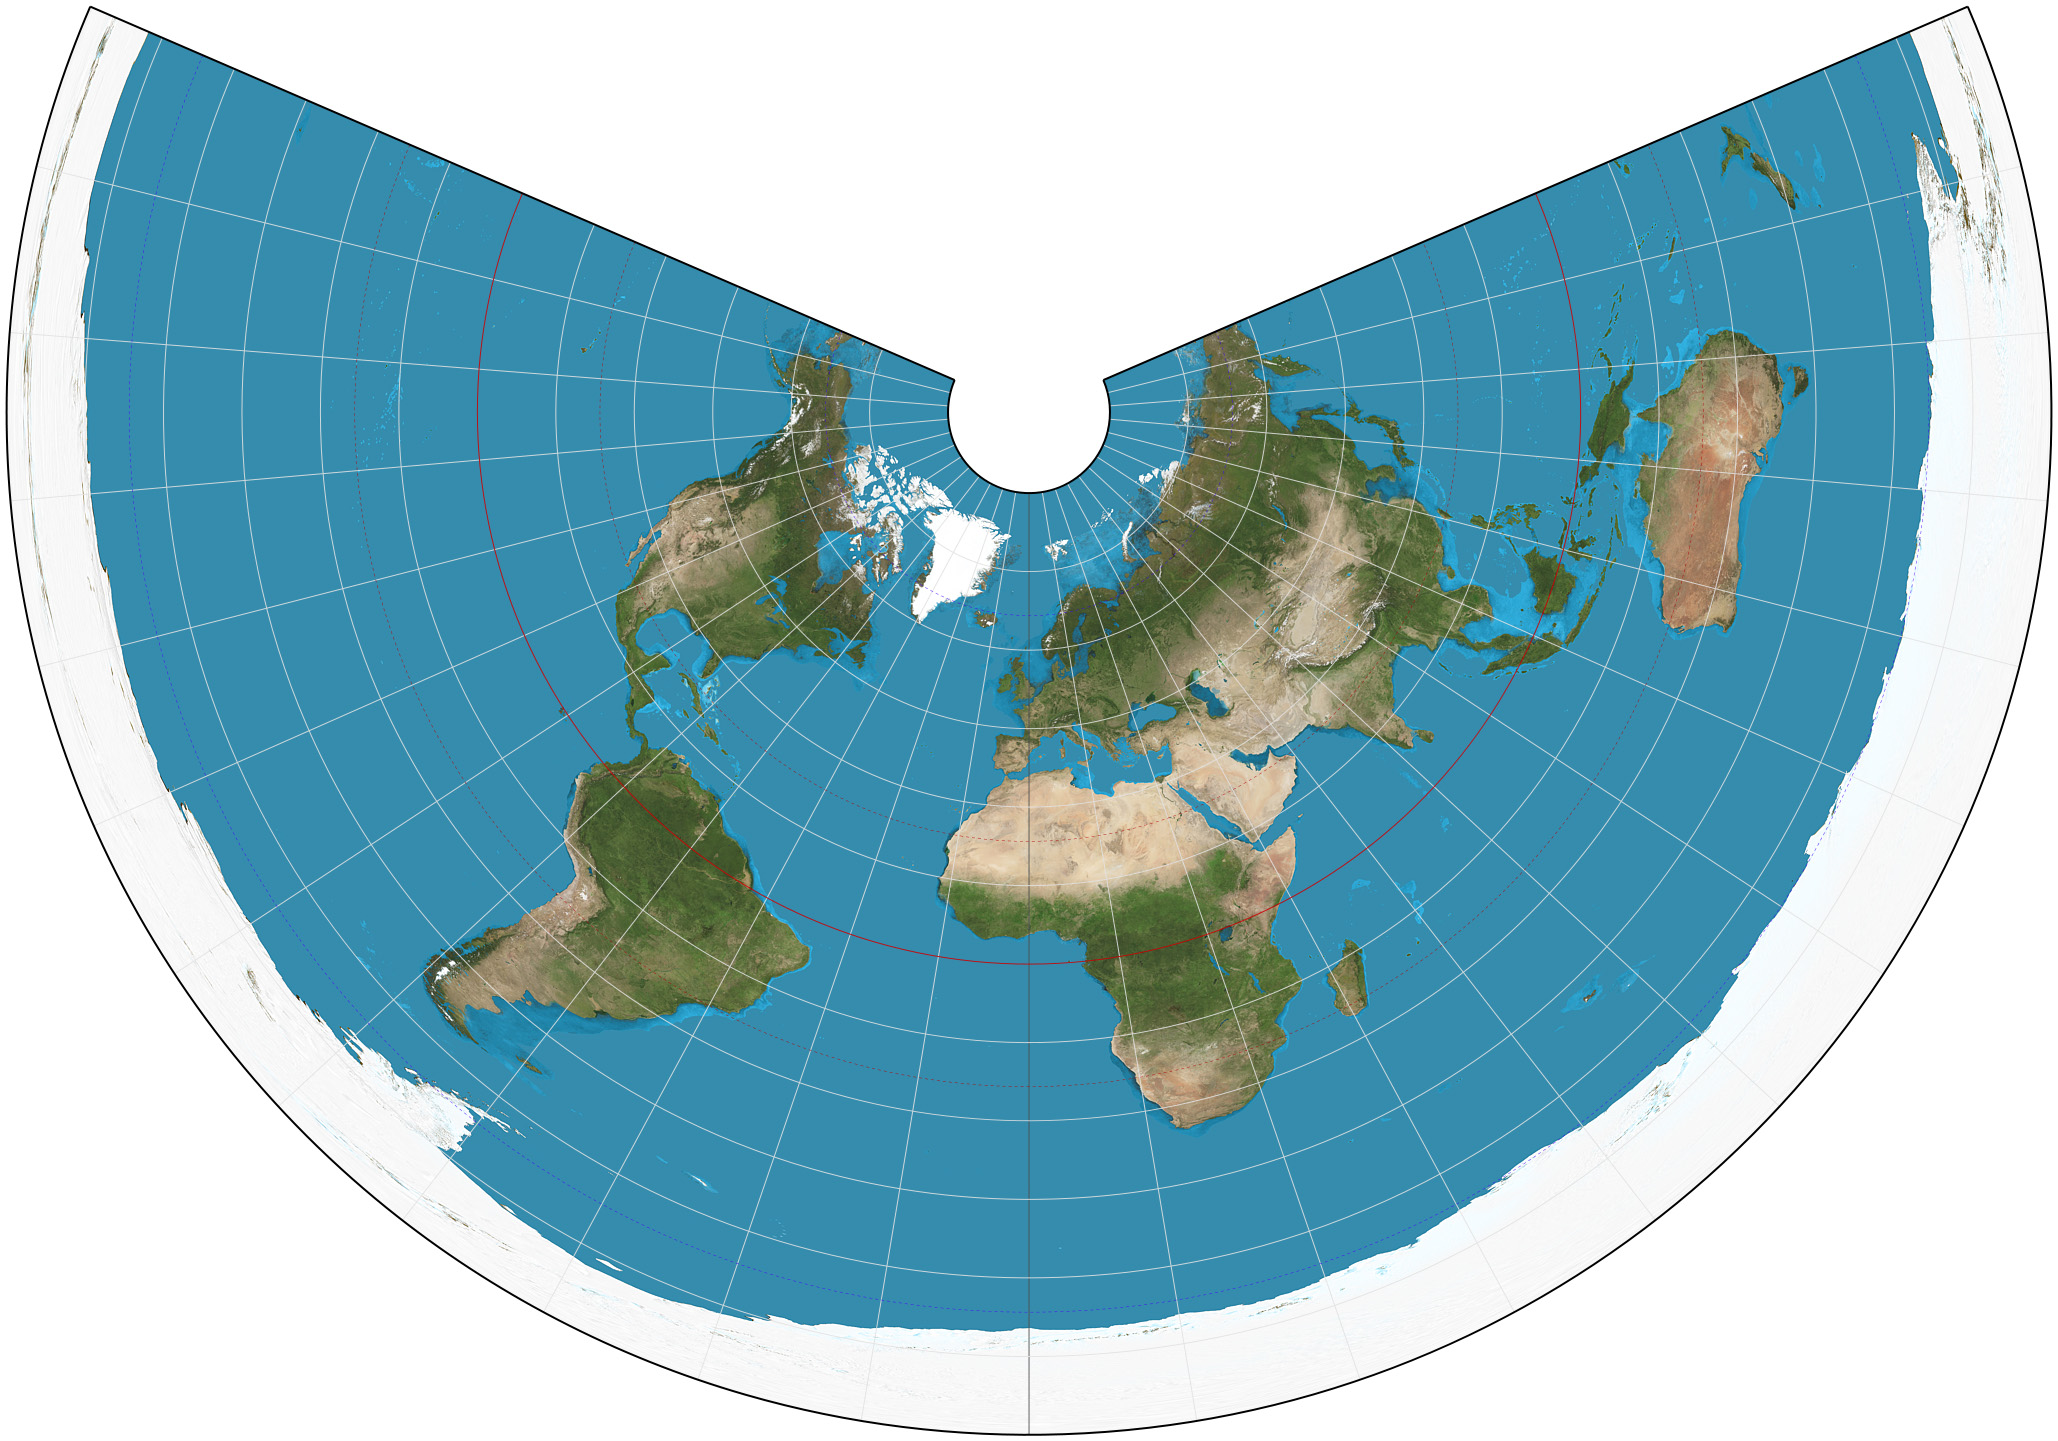
\includegraphics[height=5cm,keepaspectratio]{images/methods/projections/equidistant.jpg}
\caption[
    Equidistant conic projection, Urldate: 07.2016 \newline
    \small\texttt{\url{https://upload.wikimedia.org/wikipedia/commons/d/d8/Equidistant_conic_projection_SW.JPG}}.
]{Equidistant conic projection}
\label{fig:projections-equidistant}
\end{figure}

\end{enumerate}
\subsubsubsection{Azimuthal and related map projections}
Even though cylindrical and conic projections are related to cylinders and cones wrapped around the globe, azimuthal projections are mapped onto a plane. This plane usually is placed tan­gen­ti­al at either pole, the equator, or any intermediate point. Each placement bears a different name and are called polar, equatorial and oblique aspects respectively. This type of projection attracted attention with the rise of radio transmission. This is due to the fact, that those type of projections show the direction from the center of the projection to any other point on the map correctly. Figure \ref{fig:projections-azimuthal} on page \pageref{fig:projections-azimuthal} illustrates a polar azimuthal projection. All meridians are straight lines and radiate at their true angles from the center, whereas parallels are concentric circles. Most azimuthal projections do not have standard parallels or standard meridians, because each map has only one standard point. Azimuthals are not suitable for regions with predominant expanse in one direction, because they will maximize distortion \iacite{Snyder1987}.

\begin{figure}[!htb]
\centering
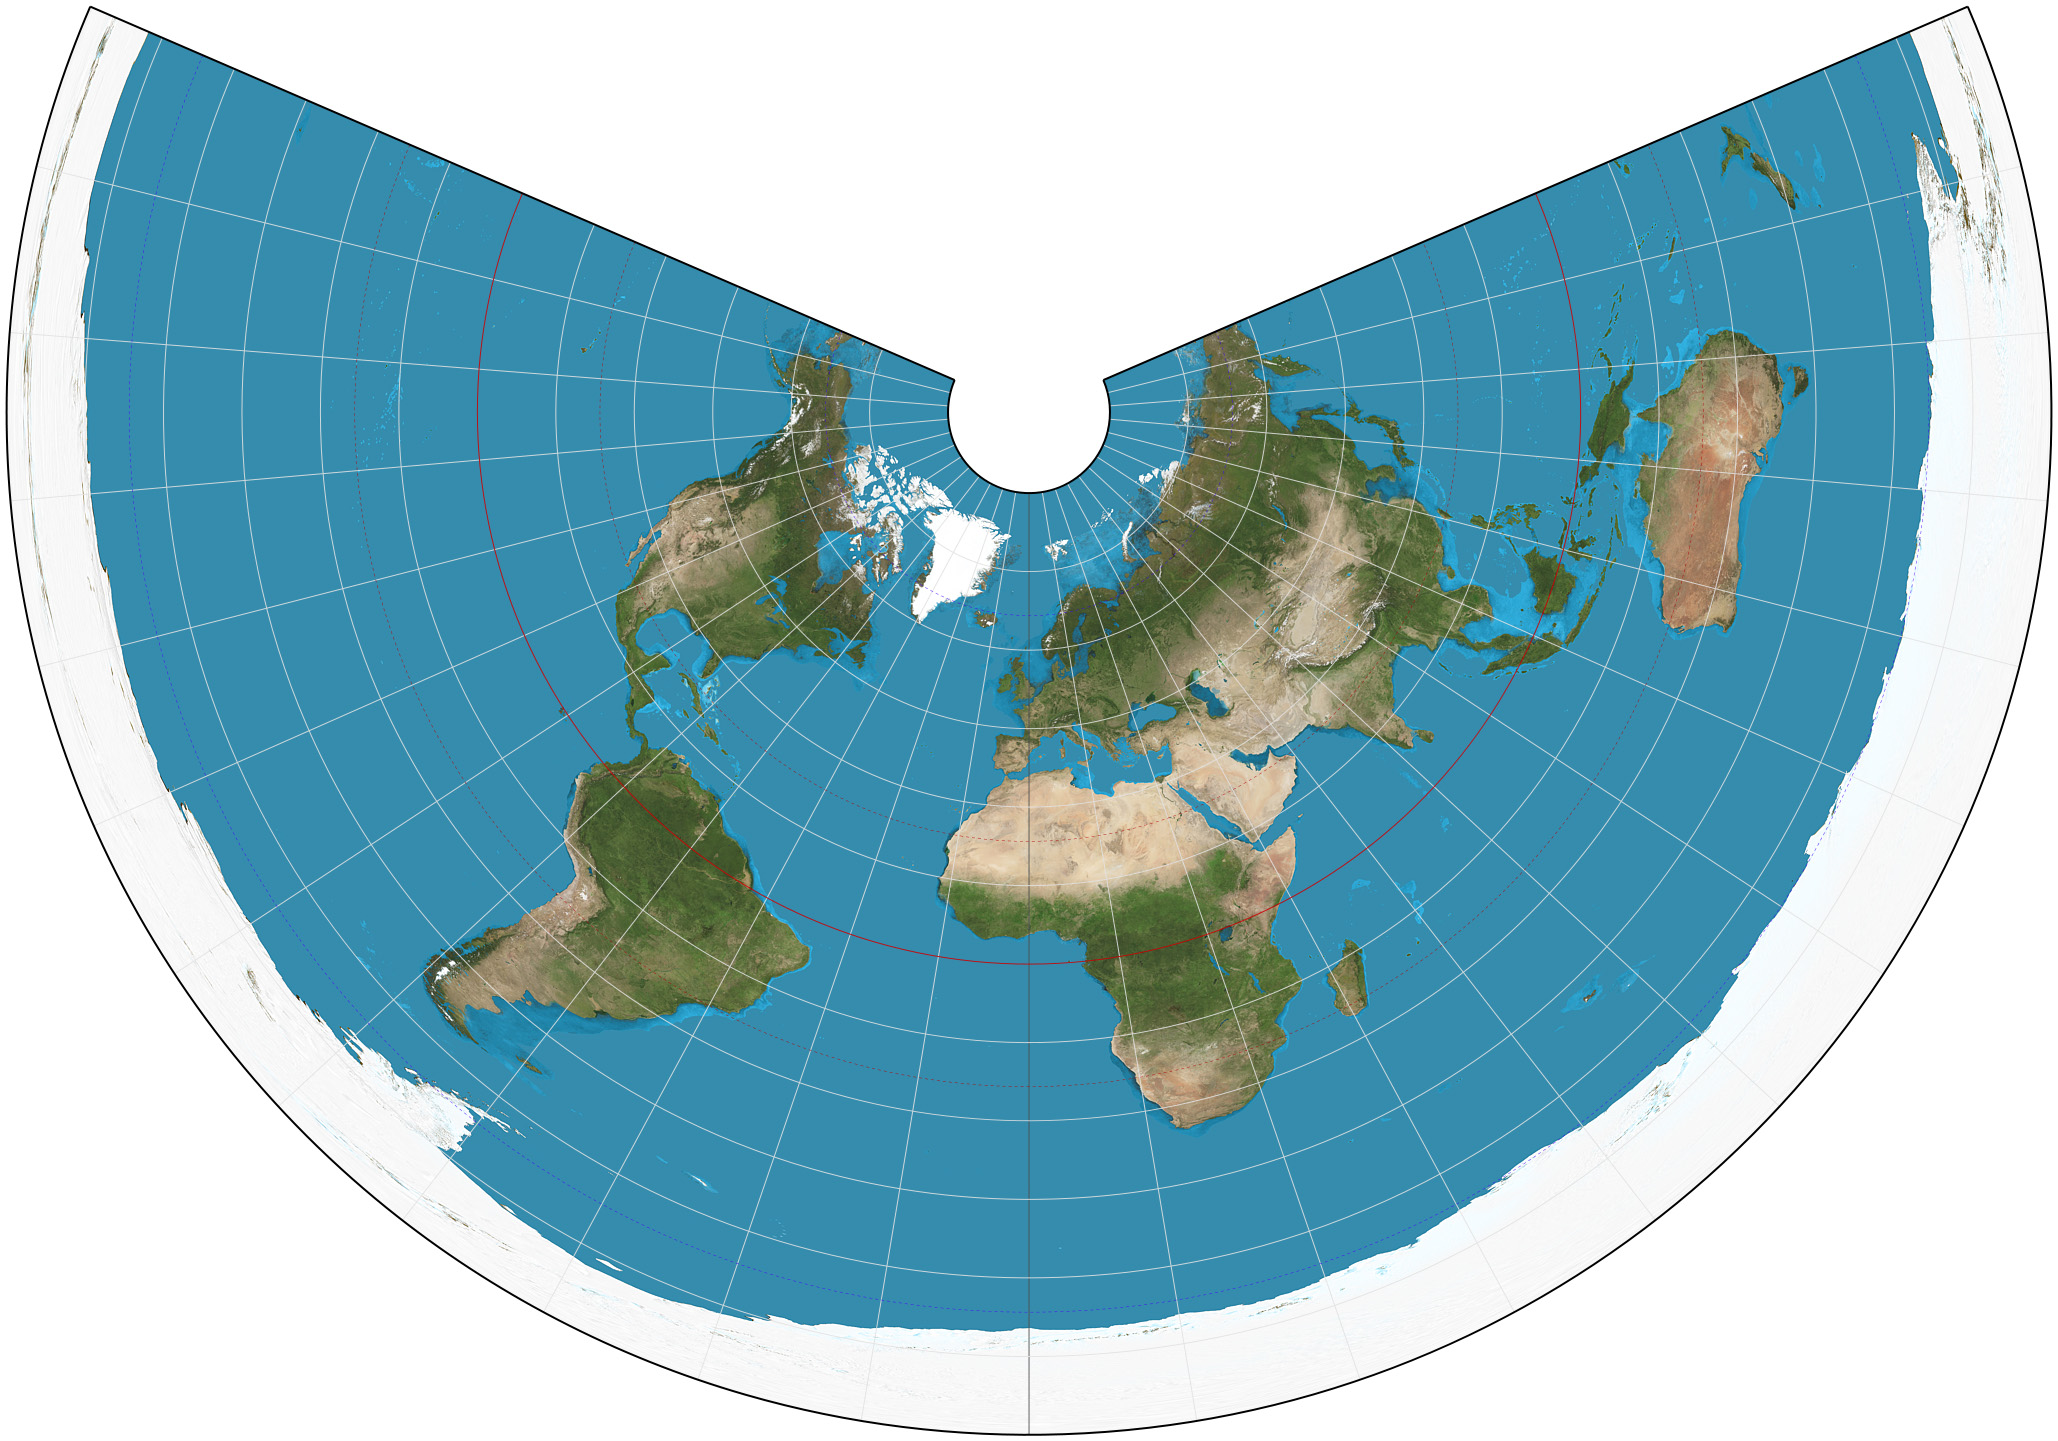
\includegraphics[height=5cm,keepaspectratio]{images/methods/projections/equidistant.jpg}
\caption[
    Azimuthal projection, Urldate: 07.2016 \newline
    \small\texttt{\url{https://upload.wikimedia.org/wikipedia/commons/e/ec/Azimuthal_equidistant_projection_SW.jpg}}.
]{Azimuthal projection}
\label{fig:projections-azimuthal}
\end{figure}